\documentclass{article}

\usepackage{amsthm}
\usepackage{amsfonts}
\usepackage{amsmath}
\usepackage{amssymb}
\usepackage{fullpage}
\usepackage{graphicx}
\usepackage[usenames]{color}
\usepackage{hyperref}
  \hypersetup{
    colorlinks = true,
    urlcolor = blue,       % color of external links using \href
    linkcolor= blue,       % color of internal links 
    citecolor= blue,       % color of links to bibliography
    filecolor= blue,        % color of file links
    }
    
\usepackage{listings}

\definecolor{dkgreen}{rgb}{0,0.6,0}
\definecolor{gray}{rgb}{0.5,0.5,0.5}
\definecolor{mauve}{rgb}{0.58,0,0.82}

\lstset{frame=tb,
  language=haskell,
  aboveskip=3mm,
  belowskip=3mm,
  showstringspaces=false,
  columns=flexible,
  basicstyle={\small\ttfamily},
  numbers=none,
  numberstyle=\tiny\color{gray},
  keywordstyle=\color{blue},
  commentstyle=\color{dkgreen},
  stringstyle=\color{mauve},
  breaklines=true,
  breakatwhitespace=true,
  tabsize=3
}

\theoremstyle{theorem} 
   \newtheorem{theorem}{Theorem}[section]
   \newtheorem{corollary}[theorem]{Corollary}
   \newtheorem{lemma}[theorem]{Lemma}
   \newtheorem{proposition}[theorem]{Proposition}
\theoremstyle{definition}
   \newtheorem{definition}[theorem]{Definition}
   \newtheorem{example}[theorem]{Example}
\theoremstyle{remark}    
  \newtheorem{remark}[theorem]{Remark}


\title{CPSC-402 Report\\Compiler Construction}
\author{Sebastian Brumm  \\ Chapman University}

\date{\today}

\begin{document}

\maketitle

\begin{abstract}
\end{abstract}

\tableofcontents

\section{Introduction}\label{intro}

This report starts with our weekly homework, which mainly includes finite state automata, abstract syntax trees, and type-checking. The second half of this report focuses on my final project, which is compiling C++ into assembly language. I decided to take this further by looking at a very basic example of a linked list in assembly.

\subsubsection{Definitons, Examples, Theorems, Etc}

\section{Homework}\label{homework}

\subsection{Week 1}

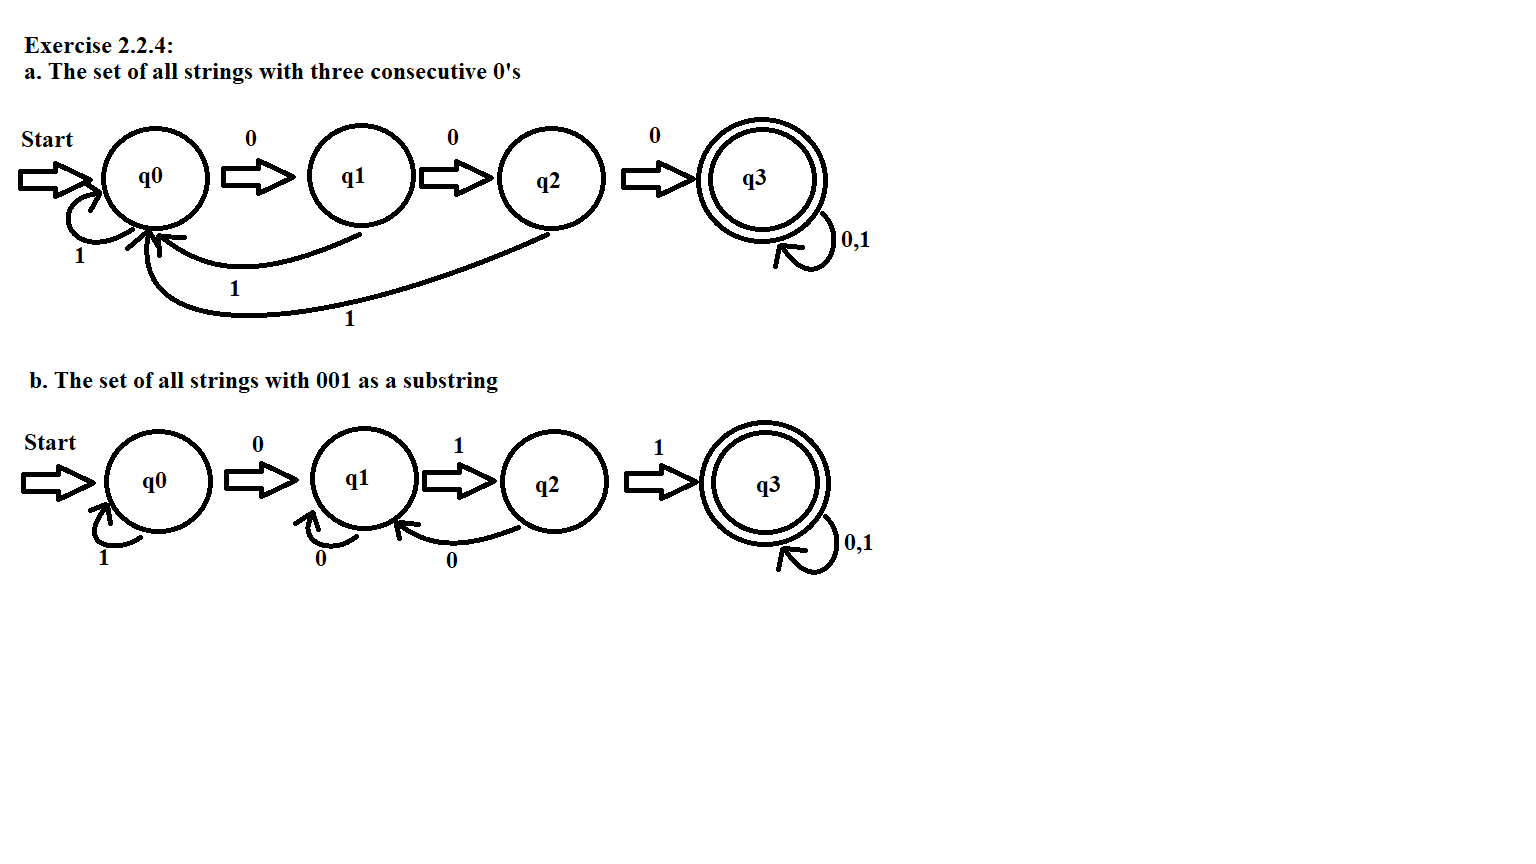
\includegraphics[scale=0.4]{Images/Homework1.png}

\subsection{Week 2}

\subsubsection{2.3.4-a: The set of all strings {0-9} such that the final digit has appeared before}
Regular Expression: $\Sigma^*0\Sigma^*0+...$ add sigma def

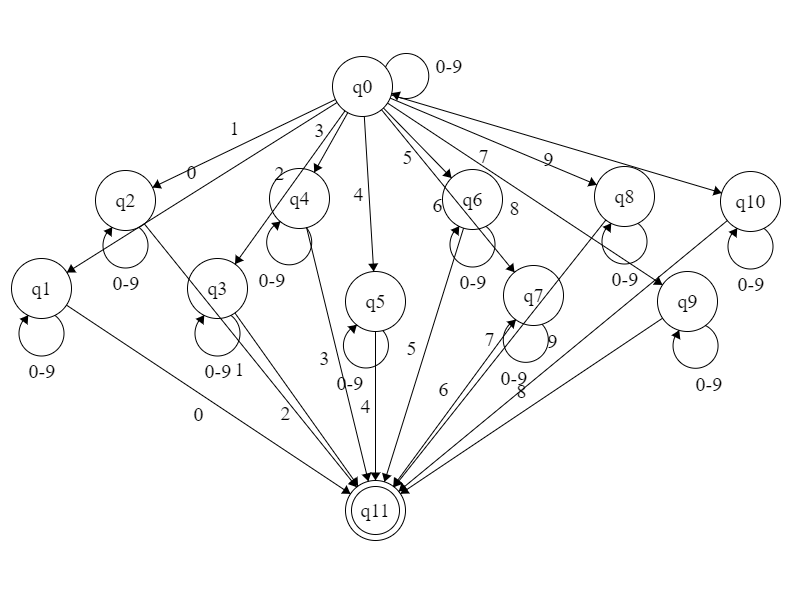
\includegraphics[scale=0.4]{Images/2.3.4a.png}

\subsubsection{2.3.4-b: The set of all strings {0-9} such that the final digit has not appeared before}
Regular Expression: $\{1-9\}0+\{0,2-9\}1...$

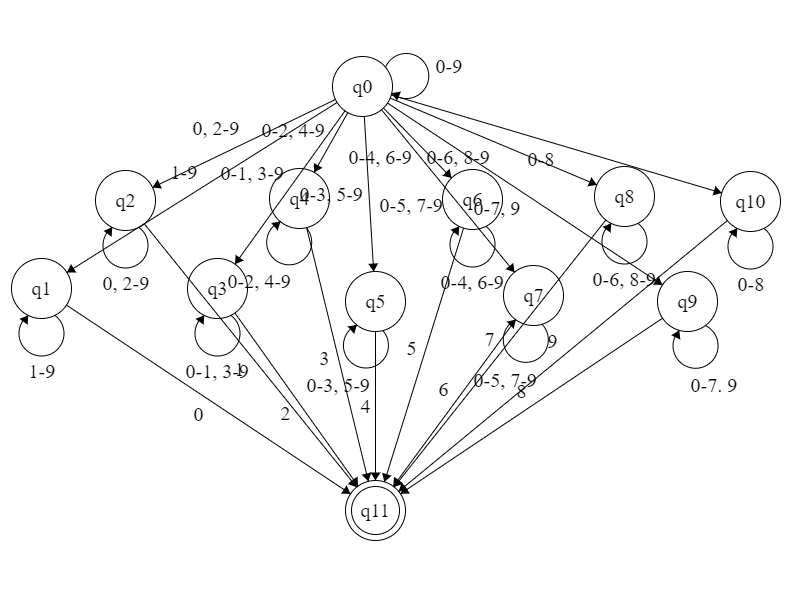
\includegraphics[scale=0.4]{Images/2.3.4b.png}

\subsubsection{2.3.4-c: The set of all strings {0,1} such that there are two 0's separated by a number of positions that is a multiple of 4, including 0}
Regular Expression: $\Sigma^*0\Sigma^{4*}0\Sigma^*$ :wrong automata, add another state after q5 with a zero transition and make it accepting

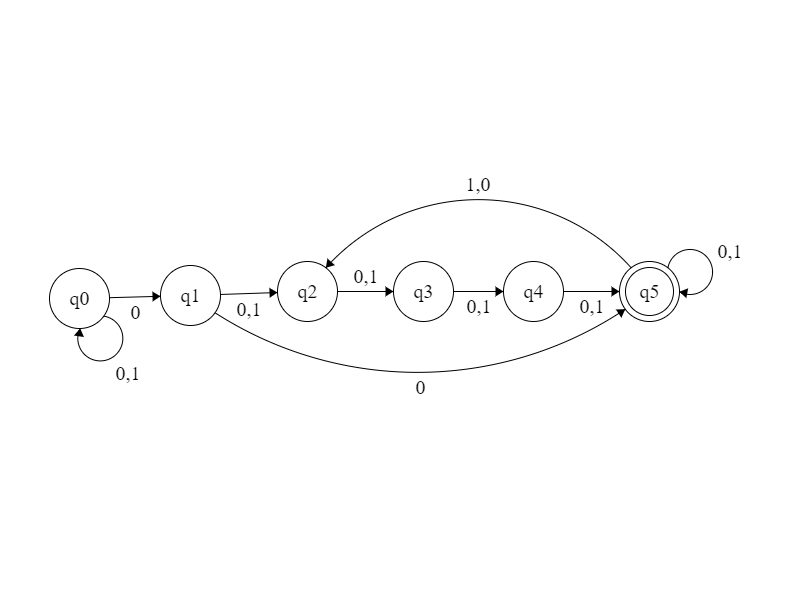
\includegraphics[scale=0.4]{Images/2.3.4c.png}

\subsubsection{2.5.3-a: The set of all strings {a,b,c} consisting of zero or more a's followed by zero or more b's followed by zero or more c's}
Regular Expression: $a^*b^*c^*$

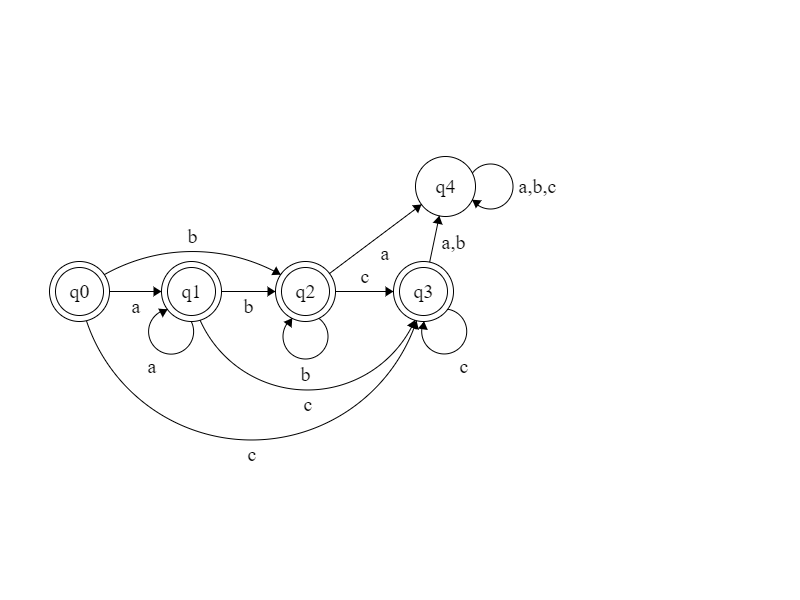
\includegraphics[scale=0.4]{Images/2.5.3a.png}

\subsubsection{2.5.3-b: The set of all strings consisting of either 01 repeated one or more times or 010 repeated one or more times}
Regular Expression: $(01)^++(010)^+$

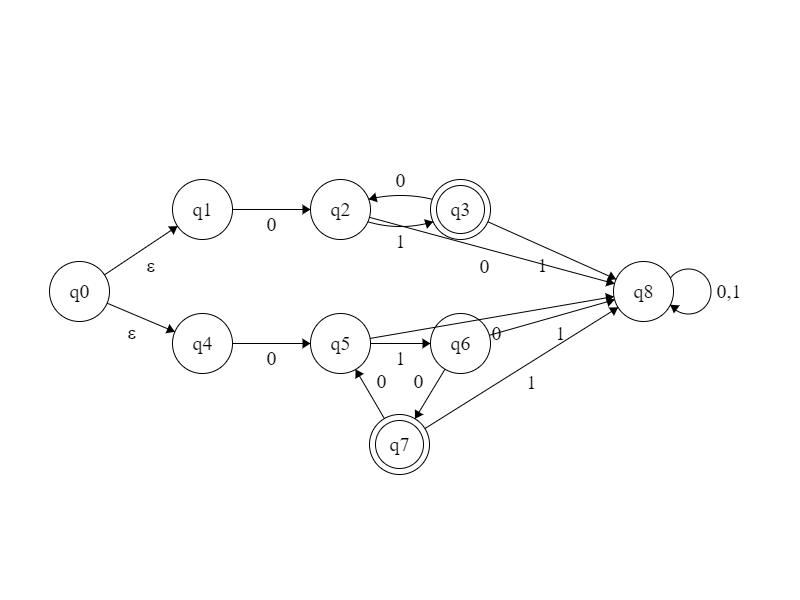
\includegraphics[scale=0.4]{Images/2.5.3b.png}

\subsubsection{2.5.3-c: The set of all strings {0,1} where at least one of the last ten positions is a 1}
Regular Expression: $\Sigma^*1\Sigma^9+\Sigma^*1\Sigma^8...+\Sigma^*1$ : remove loop on the accept state

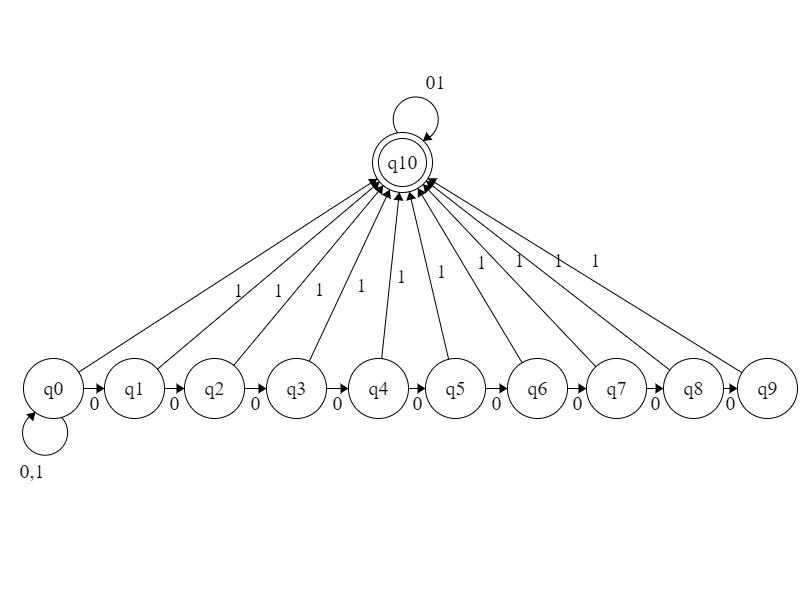
\includegraphics[scale=0.4]{Images/2.5.3c.png}

\subsection{Week 3}

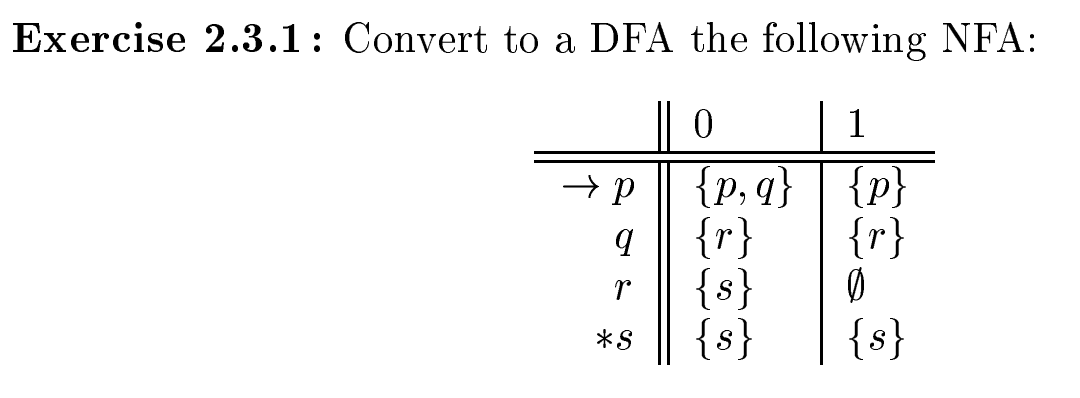
\includegraphics[scale=0.2]{Images/Week3.png}

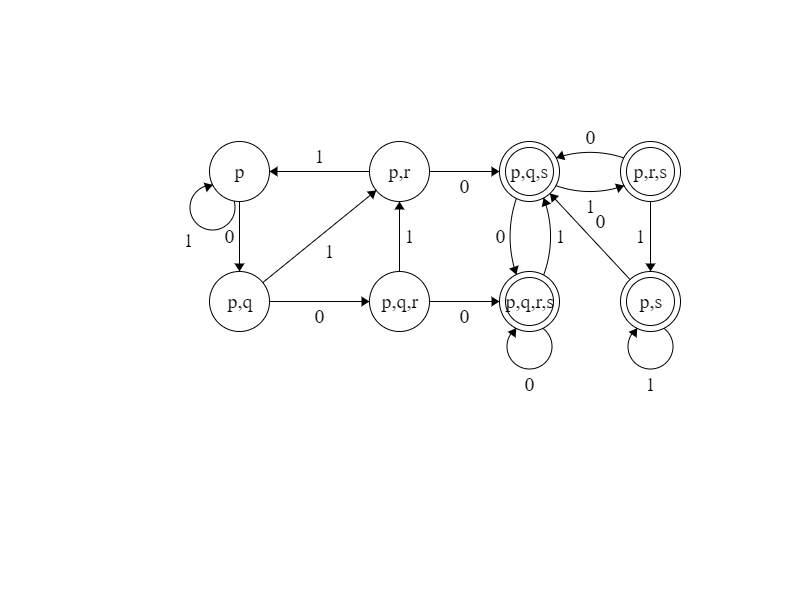
\includegraphics[scale=0.4]{Images/2.3.1.png} : change it so that pqrs -> prs on 1

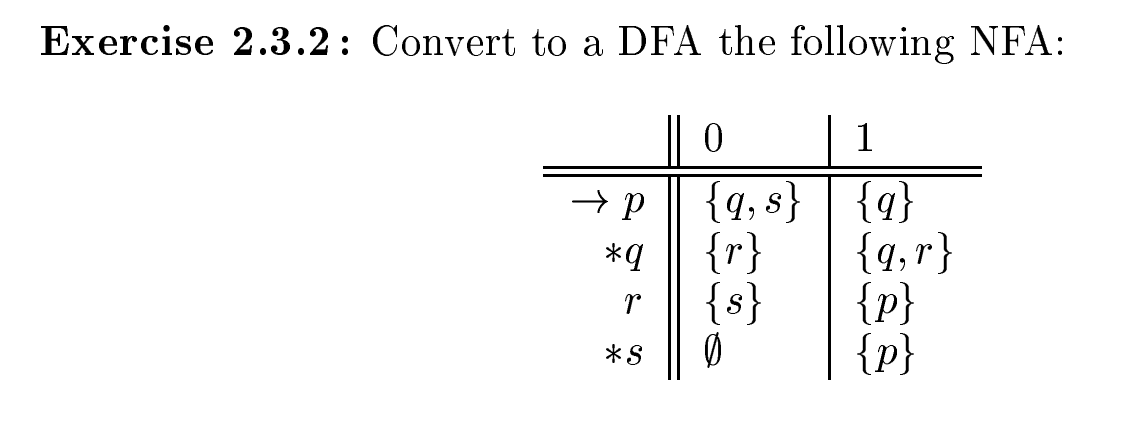
\includegraphics[scale=0.2]{Images/Week3a.png}

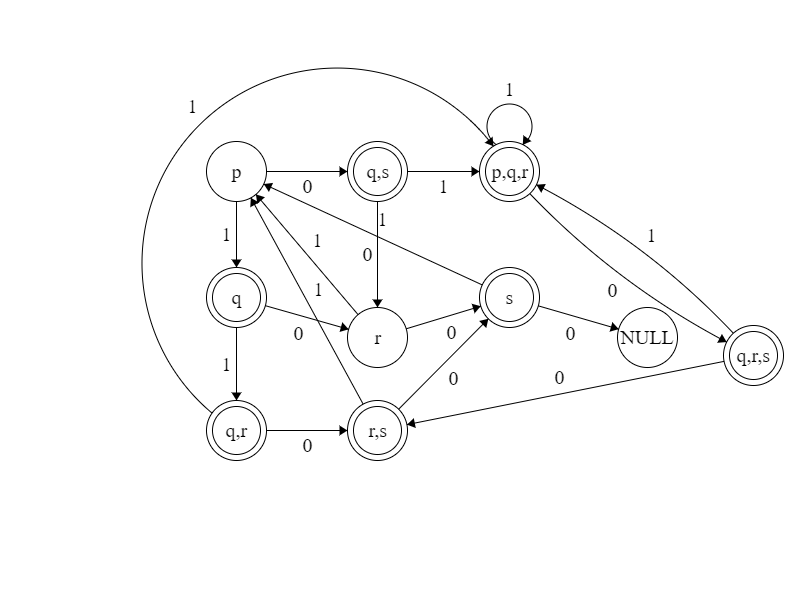
\includegraphics[scale=0.4]{Images/2.3.2.png}

\begin{lstlisting}
-- convert an NFA to a DFA
nfa2dfa :: NFA s -> DFA [s]
nfa2dfa nfa = DFA {
  -- exercise: correct the next three definitions 
  dfa_initial = [(nfa_initial nfa)],
  dfa_final = let
    final qs = disjunction (map (nfa_final nfa) qs)
    in final,
  dfa_delta = let
    delta [] c = []
    delta (q:qs) c = concat [nfa_delta nfa q c, delta qs c]
    in delta }
\end{lstlisting}

The code above is my modifications to the automata05.hs code that converts a non epsilon NFA to a DFA. I have run it with several example strings and have found it to work. The first function dfa\_initial is simple because there are no epsilon transitions here. Therefore, we can simply set the initial state of the NFA to the initial state of the DFA. If there were epsilon transitions, we would also have to account for any possible states that connect to the initial state with an epsilon transition. For the dfa\_final function, we just need to find all states that contain one of the final states from the NFA. This is done using the disjunction and map functions to find if the list of states contains an accepting state. Finally, for the dfa\_delta function, we need to recursively loop through the states that result from an input given the starting state. Both the input and output are a list of states, so we must use the concat function to keep the list as a list of states and not a list of lists.

\subsection{Week 4}

Concrete syntax tree for Fibonacci function:

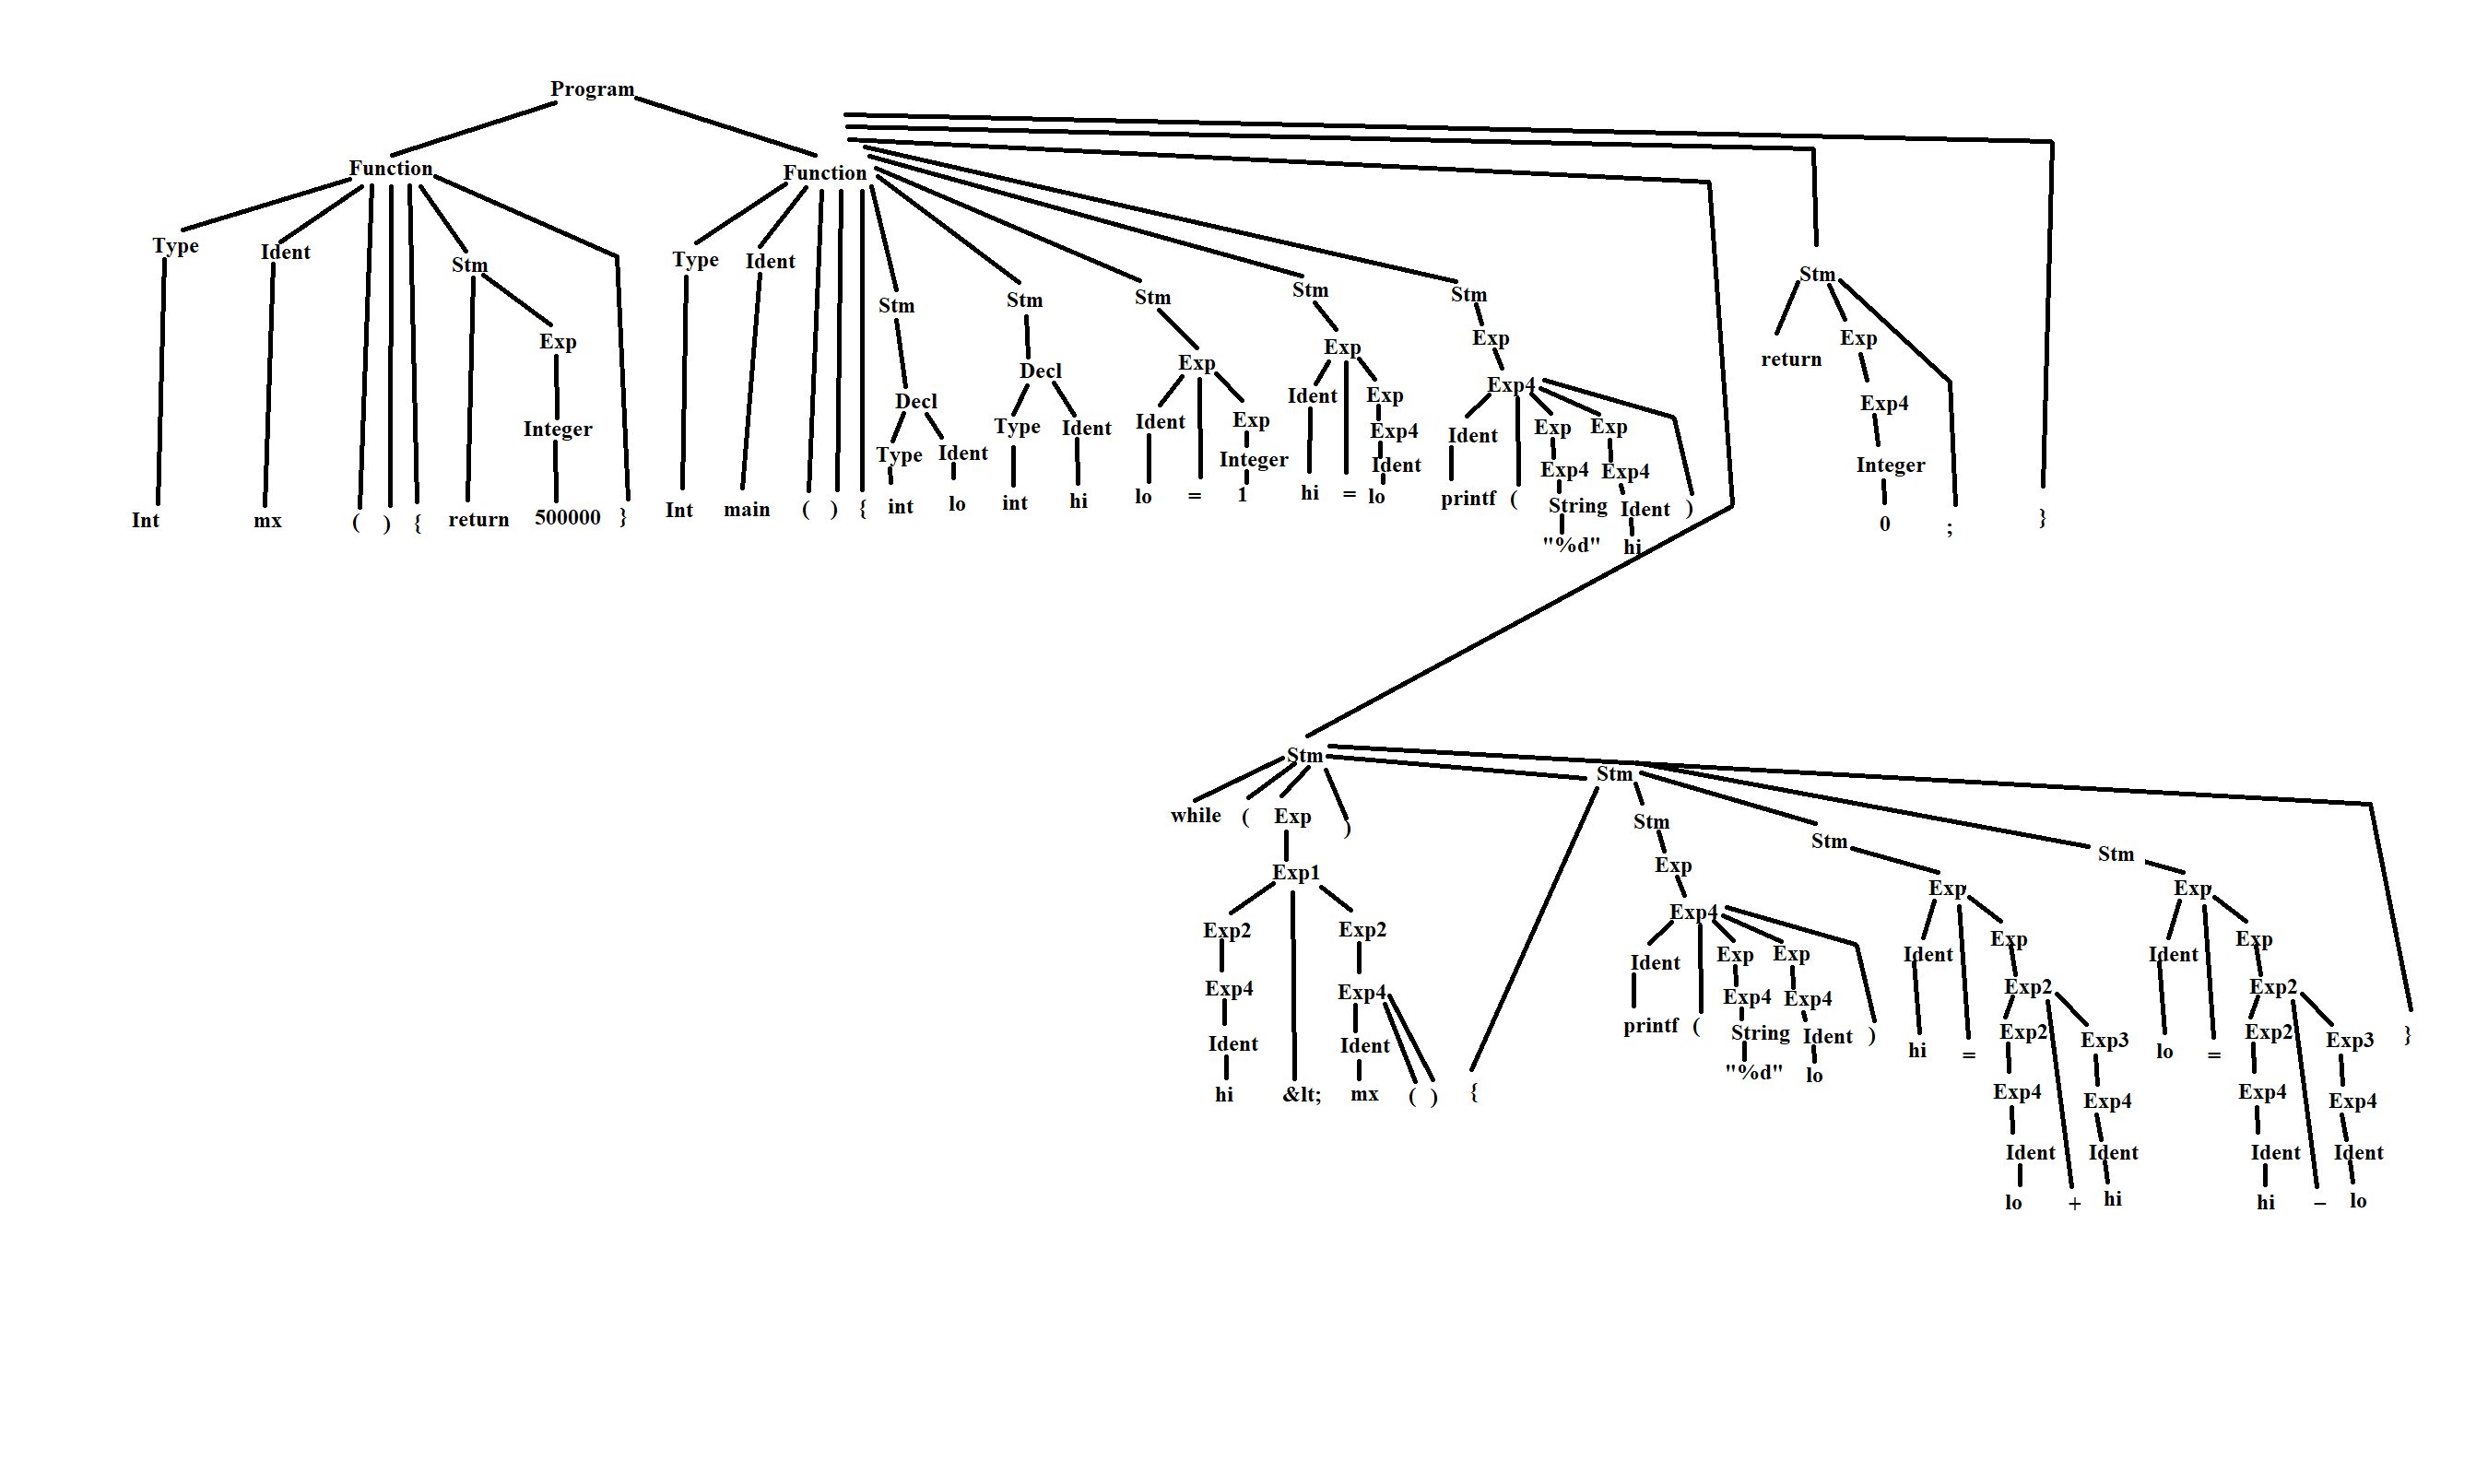
\includegraphics[scale=0.2]{Images/FibParseTree.png}

Abstract syntax tree:

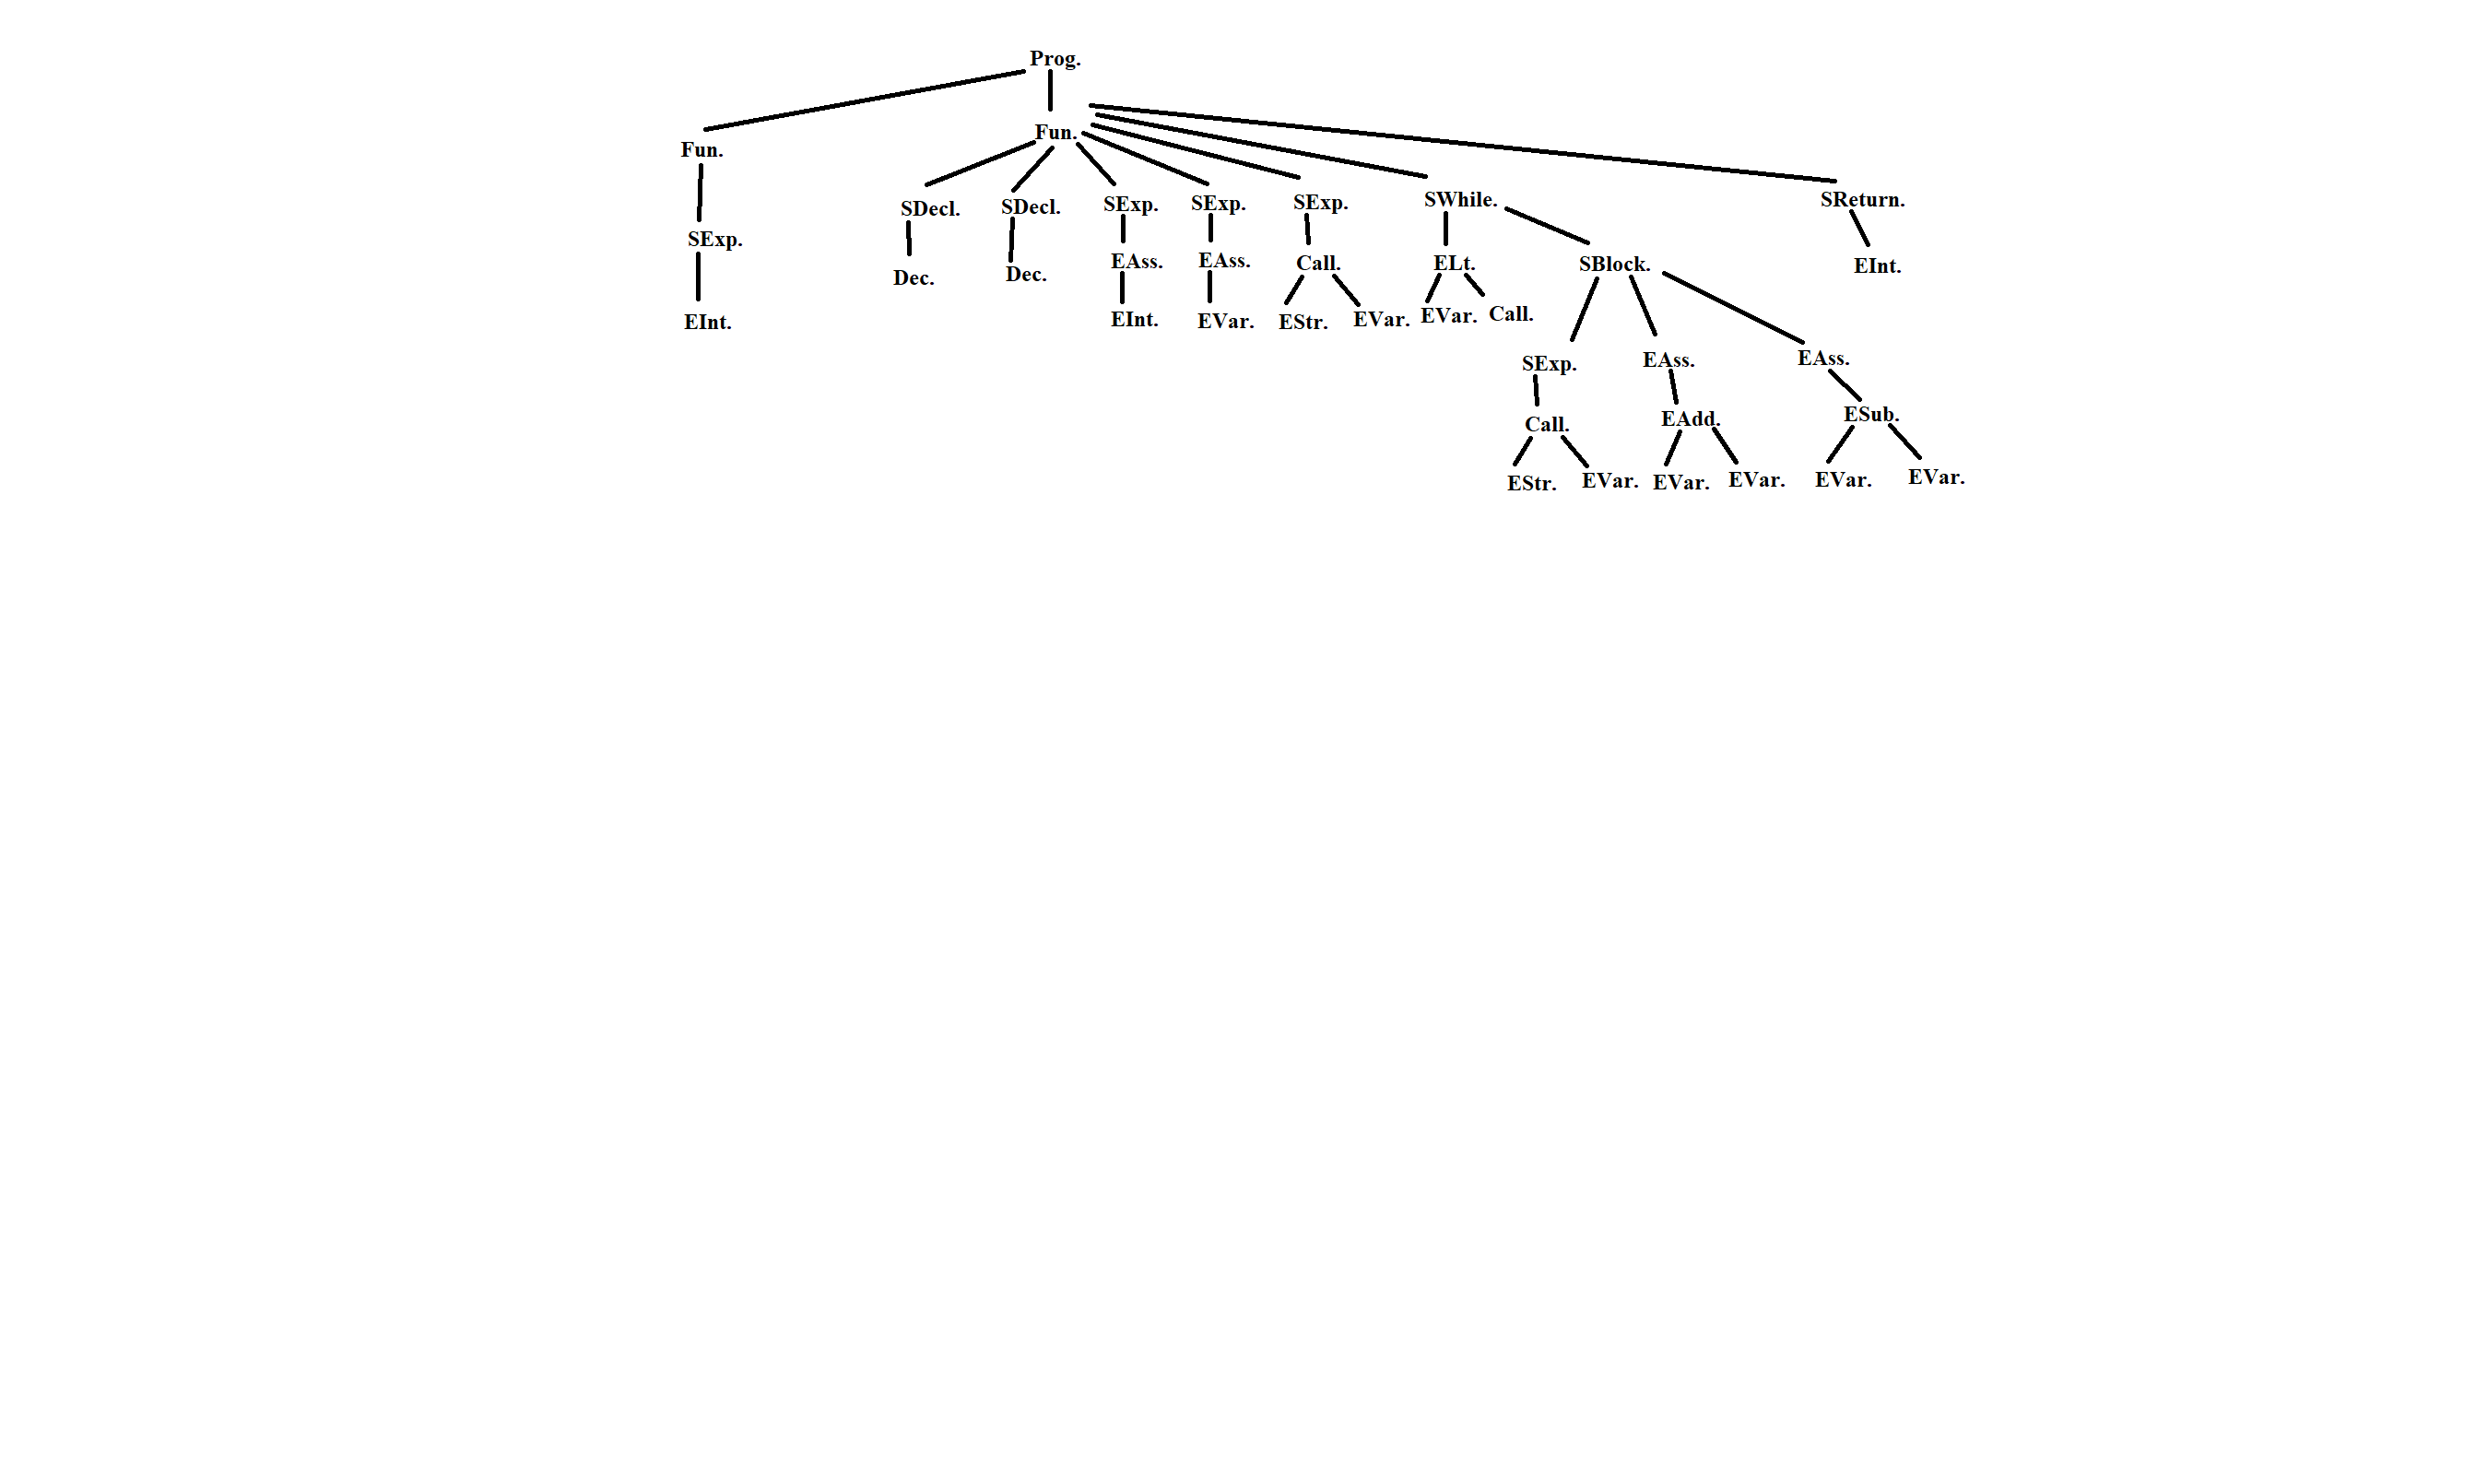
\includegraphics[scale=0.3]{Images/FibAbstractTree.png}

\subsection{Week 10}

Proof tree for the code below that the interpreter will generate:

\begin{lstlisting}
 int x ;
     {   x = 2 ;
         bool x = false && x ;
         y = y++ + ++y ; }
     x = y ;
\end{lstlisting}

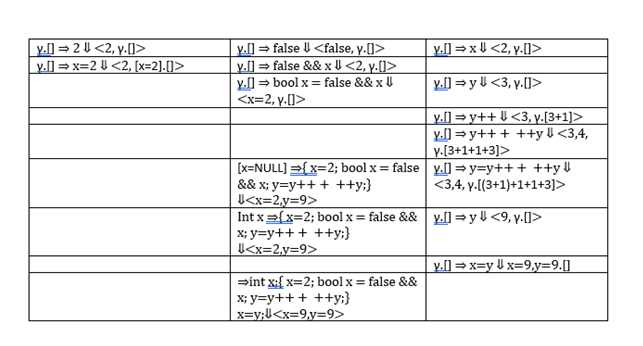
\includegraphics[scale=1.0]{Images/Week10_tree.png}

\section{Project}

\subsection{Introduction}

\par For the project, I decided to look at how C++ compiles into assembly code using the gcc compiler. I will be starting from very basic C++ operations, such as addition and assignments, and working up to showing how a very basic linked list looks in assembly. I will be using \href{https://godbolt.org/}{godbolt.org} to compile into assembly. As our first example, we can look at the  \href{https://github.com/s3t6b912/CPSC350-Assignment4/blob/master/src/ListNode.h}{ListNode.h} header file and compile it into assembly. While this is not the exact code we will be looking at later on, this is what a node from a fully functional circular linked list would work in assembly.

\begin{lstlisting}
__static_initialization_and_destruction_0(int, int):
        push    rbp
        mov     rbp, rsp
        sub     rsp, 16
        mov     DWORD PTR [rbp-4], edi
        mov     DWORD PTR [rbp-8], esi
        cmp     DWORD PTR [rbp-4], 1
        jne     .L3
        cmp     DWORD PTR [rbp-8], 65535
        jne     .L3
        mov     edi, OFFSET FLAT:_ZStL8__ioinit
        call    std::ios_base::Init::Init() [complete object constructor]
        mov     edx, OFFSET FLAT:__dso_handle
        mov     esi, OFFSET FLAT:_ZStL8__ioinit
        mov     edi, OFFSET FLAT:_ZNSt8ios_base4InitD1Ev
        call    __cxa_atexit
.L3:
        nop
        leave
        ret
_GLOBAL__sub_I_example.cpp:
        push    rbp
        mov     rbp, rsp
        mov     esi, 65535
        mov     edi, 1
        call    __static_initialization_and_destruction_0(int, int)
        pop     rbp
        ret
\end{lstlisting}

This is much less code than would typically be seen in a .cpp file because a header file is just meant to declare constructors and functions of a given class. This one in particular is shorter because there are no functions being implemented here. This class is just supposed to represent the nodes of a linked list and are not very complex. Even so, there is still a lot going on and it should be noted that the assembly code won't actually execute during compiling unless this class is called in another program. As such, we will start with more basic examples, such as return values and basic math, and then work our way up to pointers and references, which are the most important aspects of any linked list.

\subsection{The gcc Compiler}

The gcc compiler is used to compile C programs and can also compile C++ programs using the g++ call. When a user compiles a program, the first stage that the compiler takes is the preprocessing step. This is when the compiler filters out lines that start with "\#" and comments. For the former, it will include those files that are being called into the compiling, and will also define any macros that the user requests. As for comments, these are just filtered out and are not taken into consideration when compiling. The second stage is when the actual compiling occurs. The compiler will take the processed file and then compile it into assembly code. The final two stages are a out of the scope of this report, those being compiling the assembly code into binary and then linking that binary code into actual function calls that the system can execute. The result of these four stages is the output file that can be called to run the compiled program.

\subsection{Assembly Language}

Before analyzing programs in assembly, we should first discuss what assembly is and some of its syntax and inner workings. Assembly is the language in between the high-level languages that we code in, and the low-level languages that the computer can understand such as machine code and binary. It holds a strong correspondence to machine code, meaning that one statement in assembly is one instruction in machine code. Each statement is typically a mnemonic that is either built in or defined by the operating system or the user. These are also typically paired with addresses where variables are stored to and called from. It should also be noted that stacks are explicitly used to temporarily store variables and functions. These values are pushed and popped from the stack as they are called and returned.

\subsection{Basic Return and Assignment}

For this section, we will be taking a look at the below C++ code.

\begin{lstlisting}
int main() {
    int x = 1+1;
    return 0;
}
\end{lstlisting}

We will also look at this code compiled into assembly.

\begin{lstlisting}
main:
        push    rbp
        mov     rbp, rsp
        mov     DWORD PTR [rbp-4], 2
        mov     eax, DWORD PTR [rbp-4]
        pop     rbp
        ret
\end{lstlisting}

This program is simple. All it does is define a variable x as 1+1, and then it returns that variable. The assembly code is a little bit more involved and has four key functions which are called. The first, push, will decrement the stack pointer and then stores the source operand on the top of the stack. In this case, the source operand is the main function, designated as rbp in this scenario. The second line, mov, is basically an assignment. It will copy the second operand, meaning the second argument, to the first one. In other words, it is assigning the value of the second argument to the label of the first. This keyword is called three separate times in this instance. The first time is to declare the main function and assign the following statement block to it. The second time is to declare the variable "x" as "rbp-4" and assign the value of 2 to it. The last time it is called is to assign the value of x to the "return" keyword. The pop keyword is very self-explanatory. Instead of pushing to the stack, it will recieve the value that is at the top of the stack and store it in the argument, in this case being rbp, otherwise known as the main function. The last keyword, ret, will direct the program control to the return address that is located at the top of the stack. In this case, the value of rbp is at the top of the stack and this is assigned to the return value of the main function, which is this case would be 2.

\subsection{Basic Function Declaration}

For this section, we will be taking a look at the below C++ code.

\begin{lstlisting}
void empty() {}

int main() {
  empty();
  return 0;
}
\end{lstlisting}

We will also look at this code compiled into assembly.

\begin{lstlisting}
empty():
        push    rbp
        mov     rbp, rsp
        nop
        pop     rbp
        ret
main:
        push    rbp
        mov     rbp, rsp
        call    empty()
        mov     eax, 0
        pop     rbp
        ret
\end{lstlisting}

In this section we will be looking at a C++ program that contains a completely empty function in addition to the main function. The first thing to note is that these functions each have their own separate blocks of assembly code. The main function looks very similar to the last example, with one key difference, and the new empty function also is structured remarkably similar. The main function now includes the "call" keyword. This should be self-explanatory as to what it does, as it simply calls the "empty" function. More specifically, this keyword will save the procedure linking information on the stack, meaning the address of the function, and will pause running the current branch of code. The program will then transfer over to a different branch of code, in this case the one stored under "empty()", and will run the code there. Once that is done running, it will resume the main function.

Let's discuss the empty() function for a little bit. At this point, the similarities between it and the main function should be obvious. They both have the same order of push, mov, pop, and ret. This is in fact the case with all function; the main code body of the function will be sandwiched by these four keywords. In this case, we also come across the "nop" keyword. This simply lets the computer know that there is no operation to be performed, which makes sense as this is an empty function.

\subsection{Input/Ouput for Functions and For Loops}

For this section, we will be taking a look at the below C++ code.

\begin{lstlisting}
int forloop(int x) {
    int n = 0;
    for(int i = 0; i < 5; i++){
        n = n + x;
    }
    return n;
}

int main() {
  int x = 5;
  int n = forloop(x);
  return n;
}
\end{lstlisting}

We will also look at this code compiled into assembly.

\begin{lstlisting}
forloop(int):
        push    rbp
        mov     rbp, rsp
        mov     DWORD PTR [rbp-20], edi
        mov     DWORD PTR [rbp-4], 0
        mov     DWORD PTR [rbp-8], 0
        jmp     .L2
.L3:
        mov     eax, DWORD PTR [rbp-20]
        add     DWORD PTR [rbp-4], eax
        add     DWORD PTR [rbp-8], 1
.L2:
        cmp     DWORD PTR [rbp-8], 4
        jle     .L3
        mov     eax, DWORD PTR [rbp-4]
        pop     rbp
        ret
main:
        push    rbp
        mov     rbp, rsp
        sub     rsp, 16
        mov     DWORD PTR [rbp-4], 5
        mov     eax, DWORD PTR [rbp-4]
        mov     edi, eax
        call    forloop(int)
        mov     DWORD PTR [rbp-8], eax
        mov     eax, DWORD PTR [rbp-8]
        leave
        ret
\end{lstlisting}

We are now going to take the complexity of the program to the next level. We are introducing now a function that takes an input, runs through a for loop, and returns an output. This drastically increases the complexity of the assembly code, but it still largely uses the same keywords as before, in the same way as before.

Going out of order for a little bit, we will still look at the main function first. The only differences between this one and the last example is that we are assigning an additional variable, and creating a variable that is assigned the output of the forloop() function. The first thing to notice is that we have a new keyword, the sub keyword. Unsurprisingly, this stands for subtract and will simply subtract the value of the second argument from the value of the first argument. In this case, it is being applied to the main function and discussing specifically why is out of the scope of this report. The most important line in the main function is "int n = forloop(x)". This is associated with four lines in the assembly code, those being two assignments, a function call, followed by another assignment. Basically, this is copying the value of the x variable into the location of the returned value of the forloop() function, then copying this address into the actual forloop() function, calling the function to run through its branches, then finally assigning the output of the function to the variable n. Its all rather complex memory shenanigans, and we will find out later that the referenced "eax" here is the same address that the forloop() function actually returns.

Looking closer at the forloop() function itself, we can see that it has three different branches associated with it. There are also a few new keywords, of which "add" should not need to be explained. For the purposes of this report, I will only explain what the new keywords do and the general flow of this function. The "jmp" keyword simply jumps to another branch, in this case being the .L2 branch. The "cmp" keyword is the comparison operator. This correlates to the i < 5 in the for loop and will return a flag based on whether the condition is met. This flag is stored into a register and then later accessed by the "jle" keyword. This keyword will check the flags in the register and decide if it needs to jump to the designated branch. This basically describes the functionality of the for loop. The loop will keep running as long as the condition is met, and will stop running once the condition is no longer being met. The function that updates the for loop condition also occurs in this same branch.

\subsection{While Loop}

For this section, we will be taking a look at the below C++ code.

\begin{lstlisting}
/* Fibonacci */

int main () {
  int lo,hi,mx ;
  lo = 1 ;
  hi = lo ;
  mx = 5000000 ;
  //printInt(lo) ;
  while (hi < mx) {
    //printInt(hi) ;
    hi = lo + hi ;
    lo = hi - lo ;
  }
  return 0 ;

}
\end{lstlisting}

We will also look at this code compiled into assembly.

\begin{lstlisting}
main:
        push    rbp
        mov     rbp, rsp
        mov     DWORD PTR [rbp-4], 1
        mov     eax, DWORD PTR [rbp-4]
        mov     DWORD PTR [rbp-8], eax
        mov     DWORD PTR [rbp-12], 5000000
        jmp     .L2
.L3:
        mov     eax, DWORD PTR [rbp-4]
        add     DWORD PTR [rbp-8], eax
        mov     eax, DWORD PTR [rbp-8]
        sub     eax, DWORD PTR [rbp-4]
        mov     DWORD PTR [rbp-4], eax
.L2:
        mov     eax, DWORD PTR [rbp-8]
        cmp     eax, DWORD PTR [rbp-12]
        jl      .L3
        mov     eax, 0
        pop     rbp
        ret
\end{lstlisting}

After explaining how the for loop functions in assembly code, it should be immediately apparent that the while loop functions in almost exactly the same way. The code will jump to a conditional branch once it reaches the while loop and then jump to the branch that contains the actual body of the while loop. We do however see a new keyword, "jl", which is another form of the jump command and will check the condition register to see if there is a flag there that meets the condition and will jump if it does. This small program as a whole mirrors the classic Fibonacci sequence, but there is no recursion used here. It should also be noted that there is no assembly code correlating to the line int lo,hi,mx. This is because only the types of these variables are being declared, there is no actual value associated with them until later in the program.

\subsection{Pointers and References}

For this section, we will be taking a look at the below C++ code.

\begin{lstlisting}
int main ()
{
  int firstvalue, secondvalue;
  int * mypointer;

  mypointer = &firstvalue;
  *mypointer = 10;
  mypointer = &secondvalue;
  *mypointer = 20;
  return 0;
}
\end{lstlisting}

We will also look at this code compiled into assembly.

\begin{lstlisting}
main:
        push    rbp
        mov     rbp, rsp
        lea     rax, [rbp-12]
        mov     QWORD PTR [rbp-8], rax
        mov     rax, QWORD PTR [rbp-8]
        mov     DWORD PTR [rax], 10
        lea     rax, [rbp-16]
        mov     QWORD PTR [rbp-8], rax
        mov     rax, QWORD PTR [rbp-8]
        mov     DWORD PTR [rax], 20
        mov     eax, 0
        pop     rbp
        ret
\end{lstlisting}

Before we talk about the assembly code, lets first discuss what the C++ code even does. This is a simple program that will declare two integer variables and a pointer variable of type integer. The pointer is then assigned the references of each of the integer variables, where it then sets that reference to a value 10 and 20 respectively. While pointers are usually used in more complex ways, this example is enough to explain their general functionality and how this translates to assembly.

As for the assembly code, we have yet another new keyword. The "lea" keyword will store the address of the second operand into the first operand, essentially performing the function of a pointer and reference. These are correlated with the mypointer = \&firstvalue and mypointer = \&secondvalue lines of code. The assembly code also denotes exactly which variables are pointers with the inclusion of "QWORD PTR" or "DWORD PTR", depending on whether the address the pointer is pointing to is changing or the value of the address is changing.

\subsection{Linked List Nodes and Classes}

First we will look at the basic class for a node in a linked list.

\begin{lstlisting}
#include <bits/stdc++.h>
using namespace std;
  
class Node {
public:
    int data;
    Node* next;
};
\end{lstlisting}

We will also look at this code compiled into assembly.

\begin{lstlisting}
__static_initialization_and_destruction_0(int, int):
        push    rbp
        mov     rbp, rsp
        sub     rsp, 16
        mov     DWORD PTR [rbp-4], edi
        mov     DWORD PTR [rbp-8], esi
        cmp     DWORD PTR [rbp-4], 1
        jne     .L3
        cmp     DWORD PTR [rbp-8], 65535
        jne     .L3
        mov     edi, OFFSET FLAT:_ZStL8__ioinit
        call    std::ios_base::Init::Init() [complete object constructor]
        mov     edx, OFFSET FLAT:__dso_handle
        mov     esi, OFFSET FLAT:_ZStL8__ioinit
        mov     edi, OFFSET FLAT:_ZNSt8ios_base4InitD1Ev
        call    __cxa_atexit
.L3:
        nop
        leave
        ret
_GLOBAL__sub_I_example.cpp:
        push    rbp
        mov     rbp, rsp
        mov     esi, 65535
        mov     edi, 1
        call    __static_initialization_and_destruction_0(int, int)
        pop     rbp
        ret
\end{lstlisting}

Even though this code only declares a very simple class constructor, the assembly is very complex. This less has to do with the content of the class and more that a class is being declared at all. There are a lot of memory assignments that need to take place, as well as comparisons for what type of class it is, public and private variables, whether it includes other classes or objects, etc. Talking more specifically about the C++ code, all this class does is define a node that contains an integer value and a pointer. The pointer is supposed to point to the next node in the list.

We do not need to talk much more about the assembly code as most of it is memory allocation and back-end stuff. We will next look at a very simple example for how these nodes can be used.

\begin{lstlisting}
// Program to create a simple linked list with 3 nodes
int main()
{
    Node* head = NULL;
    Node* second = NULL;
    Node* third = NULL;
  
    // allocate 3 nodes in the heap
    head = new Node();
    second = new Node();
    third = new Node();
  
    head->data = 1; // assign data in first node
    head->next = second; // Link first node with
    // the second node
  
    // assign data to second node
    second->data = 2;
  
    // Link second node with the third node
    second->next = third;
  
    third->data = 3; // assign data to third node
    third->next = NULL;
    return 0;
}
\end{lstlisting}

\begin{lstlisting}
main:
        push    rbp
        mov     rbp, rsp
        sub     rsp, 32
        mov     QWORD PTR [rbp-8], 0
        mov     QWORD PTR [rbp-16], 0
        mov     QWORD PTR [rbp-24], 0
        mov     edi, 16
        call    operator new(unsigned long)
        mov     DWORD PTR [rax], 0
        mov     QWORD PTR [rax+8], 0
        mov     QWORD PTR [rbp-8], rax
        mov     edi, 16
        call    operator new(unsigned long)
        mov     DWORD PTR [rax], 0
        mov     QWORD PTR [rax+8], 0
        mov     QWORD PTR [rbp-16], rax
        mov     edi, 16
        call    operator new(unsigned long)
        mov     DWORD PTR [rax], 0
        mov     QWORD PTR [rax+8], 0
        mov     QWORD PTR [rbp-24], rax
        mov     rax, QWORD PTR [rbp-8]
        mov     DWORD PTR [rax], 1
        mov     rax, QWORD PTR [rbp-8]
        mov     rdx, QWORD PTR [rbp-16]
        mov     QWORD PTR [rax+8], rdx
        mov     rax, QWORD PTR [rbp-16]
        mov     DWORD PTR [rax], 2
        mov     rax, QWORD PTR [rbp-16]
        mov     rdx, QWORD PTR [rbp-24]
        mov     QWORD PTR [rax+8], rdx
        mov     rax, QWORD PTR [rbp-24]
        mov     DWORD PTR [rax], 3
        mov     rax, QWORD PTR [rbp-24]
        mov     QWORD PTR [rax+8], 0
        mov     eax, 0
        leave
        ret
\end{lstlisting}

Looking at this code, it's easy to see how many different assignments must be made when using even a small number of pointers. This code will simply define three nodes in the list, assign them values, and link them with the next nodes in the list. The initial declarations for each Node* can be seen starting with mov QWORD PTR [rbp-8], 0, but the declaration of new Node() has five lines of assembly code for each declaration. This is to declare a new variable, call the function, and then assign the relevant member variables before finally assigning all of that to the original variable. Assigning the "data" of the node requires an additional two moves to move to the pointer and assign the value. The "next" variable takes three moves as it has to follow an additional pointer to the next node. It's easy to see how complex the assembly code can become for fully functional linked lists, as there is a move required for every pointer and operation on that pointer.

\section{Conclusions}\label{conclusions}

A large section of the first half of this report is dedicated to finite state automata. I actually learned about these in my algoithm analysis class, so I found them to be easily understandable, but struggled more with the abstract syntax trees. I was mostly unsure about how much to include from the concrete syntax trees. When it comes to my final project, I found that assembly code was actually not as difficult to understand as I had originally thought it would be. A lot of the functions and keywords are easily understood and what their functionality is was very clear from using my chosen application. Looking further into the linked list, the amount of memory allocation that went on under the hood even for just defining a class with pointers was both surprising and not at the same time. There is a reason why we code in a more abstract language, such as C++, than assembly.

\begin{thebibliography}{99}
\bibitem[HMU]{Hopcroft}
	John E. Hopcroft, Rajeev Motwani, Jeffrey D. Ullman:
\href{http://ce.sharif.edu/courses/94-95/1/ce414-2/resources/root/Text\%20Books/Automata/John\%20E.\%20Hopcroft,\%20Rajeev\%20Motwani,\%20Jeffrey\%20D.\%20Ullman-Introduction\%20to\%20Automata\%20Theory,\%20Languages,\%20and\%20Computations-Prentice\%20Hall\%20(2006).pdf}{Introduction to automata theory, languages, and computation,} 3rd Edition. Pearson international edition, Addison-Wesley 2007

\end{thebibliography}

\end{document}
